\section{Introduction}
\label{sec:intro}

In the past year, latent diffusion models have made significant progress in text-to-image research and have generated substantial commercial value. On one hand, there is a growing consensus among researchers regarding several key points: (1) Replace U-Net with Transformer architectures~\citep{chenpixart,chen2024pixart,esser2024scaling, FLUX}, (2) Using Vision Language Models (VLM) for auto-labelling images~\citep{chenpixart,Dalle-3,zhuo2024lumina,liu2024playground} (3) Improving Variational Autoencoders (VAEs) and Text encoder~\citep{podell2023sdxl,esser2024scaling,dai2023emu} (4) Achieving ultra High-resolution image generation~\citep{chen2024pixart}, etc. On the other hand, industry models are becoming increasingly large, with parameter counts escalating from PixArt's 0.6B parameters to SD3 at 8B, LiDiT at 10B, Flux at 12B, and Playground v3 at 24B. This trend results in extremely high training and inference costs, creating challenges for most consumers who find these models difficult and expensive to use. Given these challenges, a pivotal question arises: \textit{Can we develop a high-quality and high-resolution image generator that is computationally efficient and runs very fast on both cloud and edge devices?}

\begin{figure}[htbp]
    \centering
    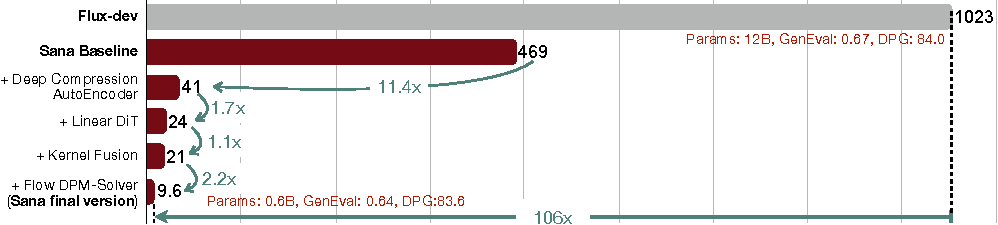
\includegraphics[width=0.99\textwidth]{figures/performance-of-different-parts.pdf}
    \caption{
    Algorithm and system co-optimize reduce the inference latency of 4096$\times$4096 image generation, from 469 seconds to 9.6 seconds, and achieve \textbf{106$\times$} faster than the current SOTA model, FLUX.
    The numbers are measured with batch size 1 on an A100 GPU.
    }
    \label{fig:speed_up}
    \vspace{-1em}
  \end{figure}


This paper proposes \model{}, a pipeline designed to efficiently and cost-effectively train and synthesize images at resolutions ranging from 1024$\times$1024 to 4096$\times$4096 with high quality. To our knowledge, no published works have directly explored 4K resolution image generation, except for PixArt-$\Sigma$~\citep{chen2024pixart}. However, PixArt-$\Sigma$ is limited to generating images close to 4K resolution (3840$\times$2160) and is relatively slow when producing such high-resolution images. To achieve this ambitious goal, we propose several core designs:

\textbf{Deep Compression Autoencoder:}
We introduce a new Autoencoder (AE) in Section \ref{vae} that aggressively increases the scaling factor to 32. In the past, mainstream AEs only compressed the image's length and width with a factor of 8 (AE-F8). Compared with AE-F8, our AE-F32 outputs 16$~\times$ fewer latent tokens, which is crucial for efficient training and generating ultra-high-resolution images, such as 4K resolution.

\textbf{Efficient Linear DiT:} 
We introduce a new linear DiT to replace vanilla quadratic attention modules (Section \ref{sec:efficient_design}). 
The computational complexity of the original DiT's self-attention is O(N$^2$), which increases quadratically when processing high-resolution images. We replace all vanilla attention with linear attention, reducing the computational complexity from O(N$^2$) to O(N).
At the same time, we propose Mix-FFN, which integrates 3$\times$3 depth-wise convolution into MLP to aggregate the local information of tokens. We argue that linear attention can achieve results comparable to vanilla attention with proper design and is more efficient for high-resolution image generation~(e.g., accelerating by 1.7$\times$ at 4K). Additionally, the indirect benefit of Mix-FFN is that we do not need position encoding~(NoPE). For the first time, we removed the positional embedding in DiT and find no quality loss.

\textbf{Decoder-only Small LLM as Text Encoder:} 
In Section~\ref{sec:text_encoder}, we utilize the latest Large Language Model~(LLM), Gemma, as our text encoder to enhance the understanding and reasoning capabilities regarding user prompts. Although text-to-image generation models have advanced significantly over the years, most existing models still rely on CLIP or T5 for text encoding, which often lack robust text comprehension and instruction-following abilities.
Decoder-only LLMs, such as Gemma, exhibit strong text understanding and reasoning capabilities, demonstrating an ability to follow human instructions effectively. In this work, we first address the training instability issues that arise from directly adopting an LLM as a text encoder. Secondly, we design complex human instructions (CHI) to leverage the LLM's powerful instruction-following, in-context learning, and reasoning capabilities to improve image-text alignment.

\textbf{Efficient Training and Inference Strategy:}
In Section \ref{data_curation}, we propose a set of automatic labelling and training strategies to improve the consistency between text and images. First, for each image, we utilize multiple VLMs to generate re-captions. Although the capabilities of these VLMs vary, their complementary strengths improve the diversity of the captions. 
In addition, we propose a clipscore-based training strategy (Section \ref{flow_schedule_train}), where we dynamically select captions with high clip scores for the multiple captions corresponding to an image based on probability.
Experiments show that this approach improve training convergence and text-image alignment. Furthermore, We propose a Flow-DPM-Solver that reduces the inference sampling steps from 28-50 to 14-20 steps compared to the widely used Flow-Euler-Solver, while achieving better results.

In conclusion, our \model{}-0.6B achieves a throughput that is over 100$\times$ faster than the current state-of-the-art method (FLUX) for 4K image generation (Figure~\ref{fig:speed_up}), and 40$\times$ faster for 1K resolution~(Figure~\ref{fig:model_size}), while delivering competitive results across many benchmarks.
In addition, we quantize \model{}-0.6B and deploy it on an edge device, as detailed in Section \ref{sec:deploy}. It takes only 0.37s to generate a 1024$\times$1024 resolution image on a customer-grade 4090 GPU, providing a powerful foundation model for real-time image generation.
We hope that our model can be efficiently utilized by all industry professionals and everyday users, offering them significant business value.
